\subsection{Muon system}

\label{sec:muon}


The muon detector will match the geometrical acceptances of the tracker and ECal, and will be about a cubic meter in size. With such 
geometrical coverage, the efficiency of detecting high mass A$^\prime$s in the $\mu^+\mu^-$ decay channel will be higher than for $e^+e^-$ 
decays, see Figure \ref{fig:muacc}. The di-muon decay channel of the A$^\prime$ has the advantage of having greatly reduced electromagnetic 
backgrounds.  In this case, the only particle background in a muon counter would come from the photoproduction of $\pi^+$ and $\pi^-$ pairs
that are not fully stopped in the ECal or absorber.  The expected low background and the high detection efficiency makes the di-muon final state an
attractive complement to the $e^+e^-$ final state. It will add substantial territory in the mass and coupling
parameter space as show in Figure \ref{fig:mureach} and will offer valuable cross-checks. With the addition of a muon system, HPS will be the 
only fixed target experiment proposed to date to search for heavy photons in an alternative to the $e^+e^-$ decay mode.

\begin{figure*}[!ht]
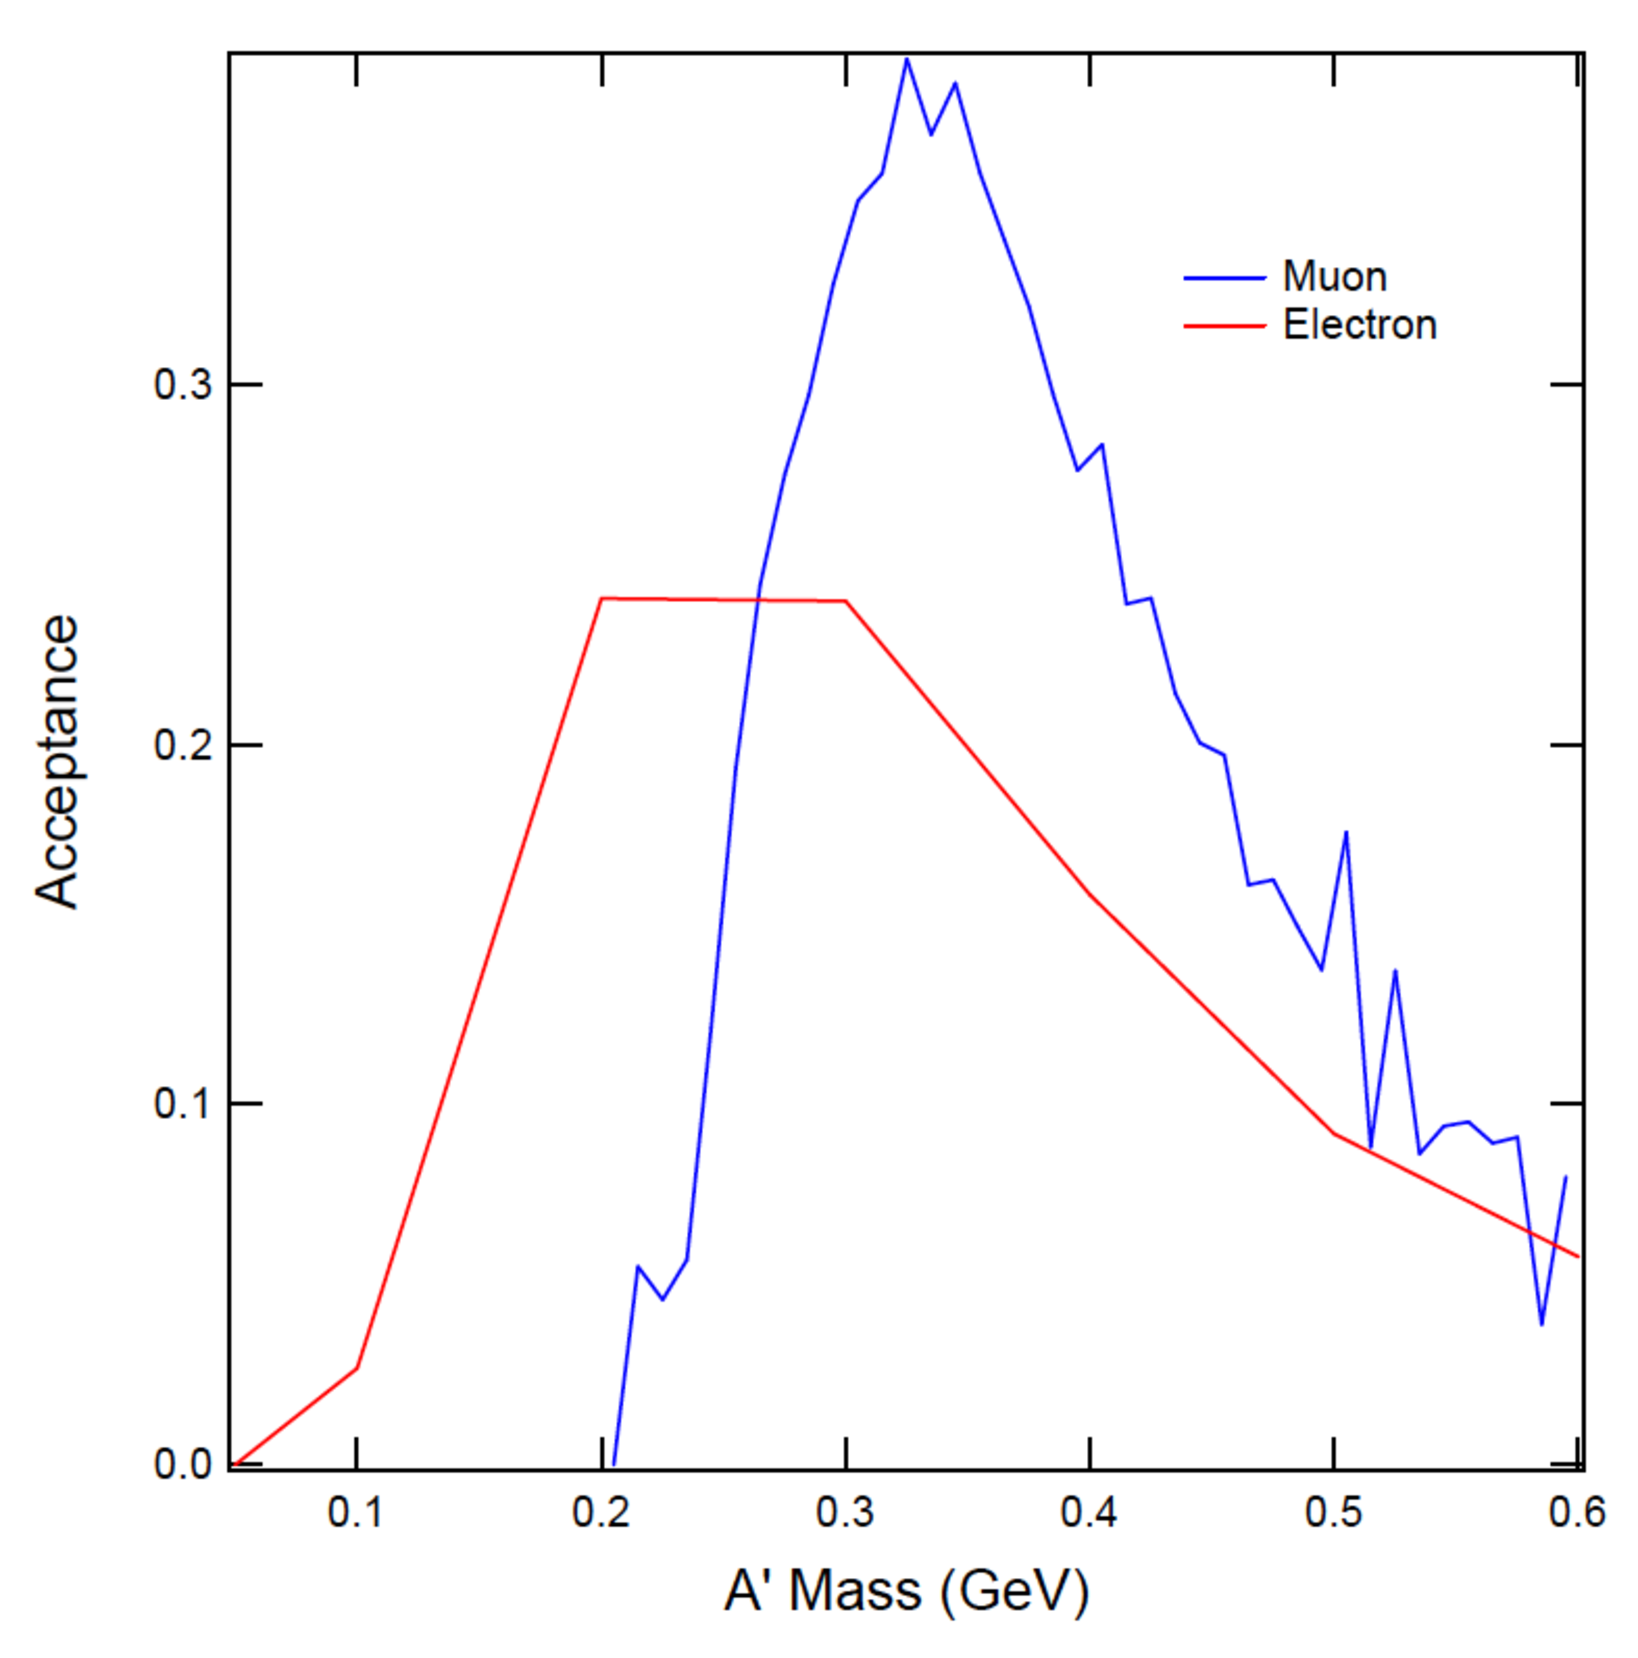
\includegraphics[scale=0.4]{muon/acc.pdf}
\caption{\small{A$^\prime$ detection efficiency through $\mu^+\mu^-$ (blue) and $e^+e^-$ (red) decay channels as a function of mass for 6.6 
GeV beam energy.}}\label{fig:muacc}
\end{figure*}

\begin{figure*}[!ht]
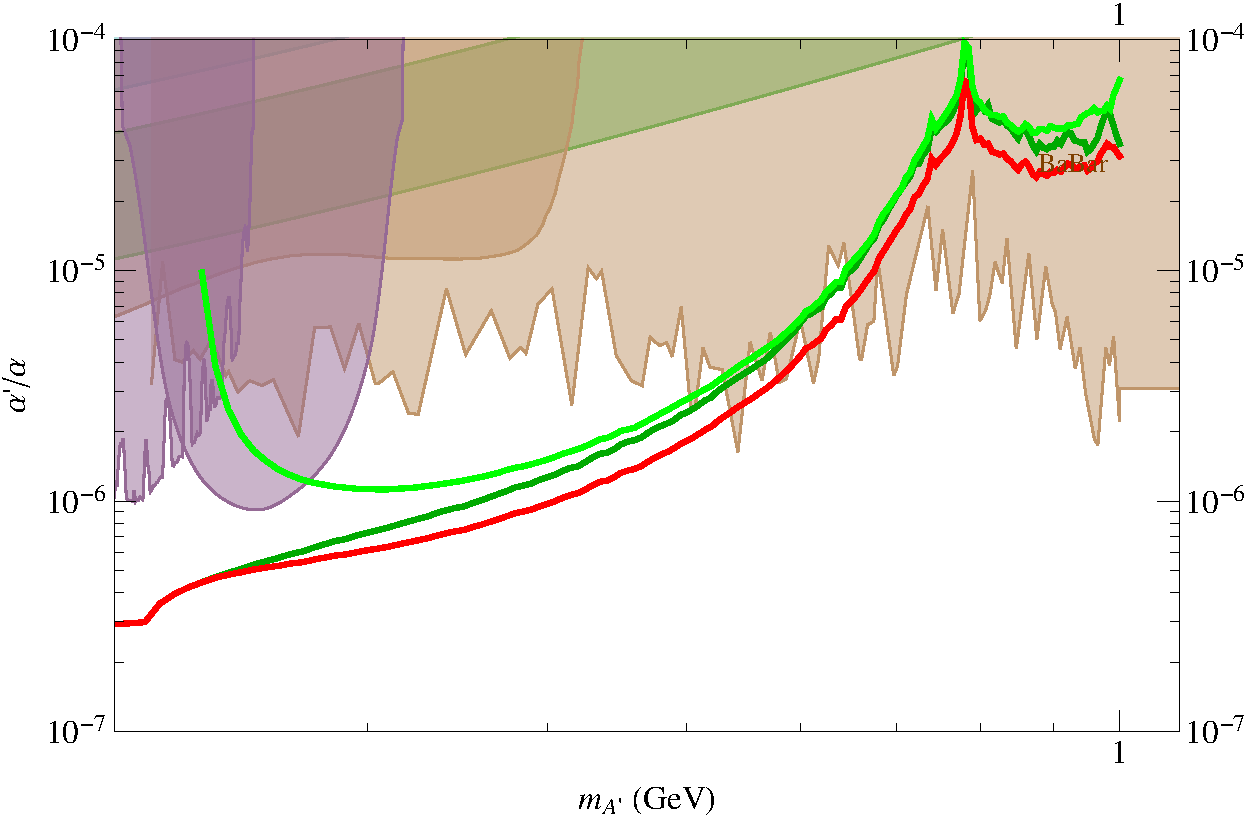
\includegraphics[scale=0.7]{muon/HPS_reach_muon.pdf}
\caption{\small{Experimental reach for 2 weeks of beam time at 6.6 GeV for $\mu^+\mu^-$ (light green) and $e^+e^-$ (dark green) decay channels. 
The red line is the combined reach.}}\label{fig:mureach}
\end{figure*}


The muon system can easily be constructed with layers of scintillator hodoscopes sandwiched between iron absorbers, and can easily be added 
downstream of the rest of the HPS apparatus.
The number of layers and the thickness of absorbers is defined by the $\pi/\mu$ rejection factor. The schematic design of the muon 
detector was optimized using the GEANT-3 model for the ECal with added layers of iron and scintillators.  In the simulation, muons 
and pions in the momentum range of $1$ to $4$ GeV/c first passed through the 16 cm of lead tungstate in the ECal and then entered a 
muon counter with various total absorber thicknesses (see \cite{HPS_PROP} for details).  Detection efficiencies for pions ($\epsilon_\pi$) 
and muons ($\epsilon_\mu$) were then calculated as a function of absorber thickness and particle momentum.  For low-energy 
particles ($< 1.7$ GeV) detection in all four layers of scintillator hodoscopes was not considered. Depending on the momentum, particles 
were not traced behind the third, fourth or fifth absorber.  
Figure \ref{fig:pmrej} shows the resulting rejection factor $\epsilon_\pi/\epsilon_\mu$.  The right-hand plot shows the
dependence of  $\epsilon_\pi/\epsilon_\mu$ on the total thickness of the iron absorber, with the best rejection at about 75 cm.  
The right-hand plot shows $\epsilon_\pi/\epsilon_\mu$ for a 75 cm absorber as a function of muon momentum.  The suppression of 
individual pions by two orders of magnitude will suppress pion pairs by 4 orders of magnitude.  

\begin{figure*}[!ht]
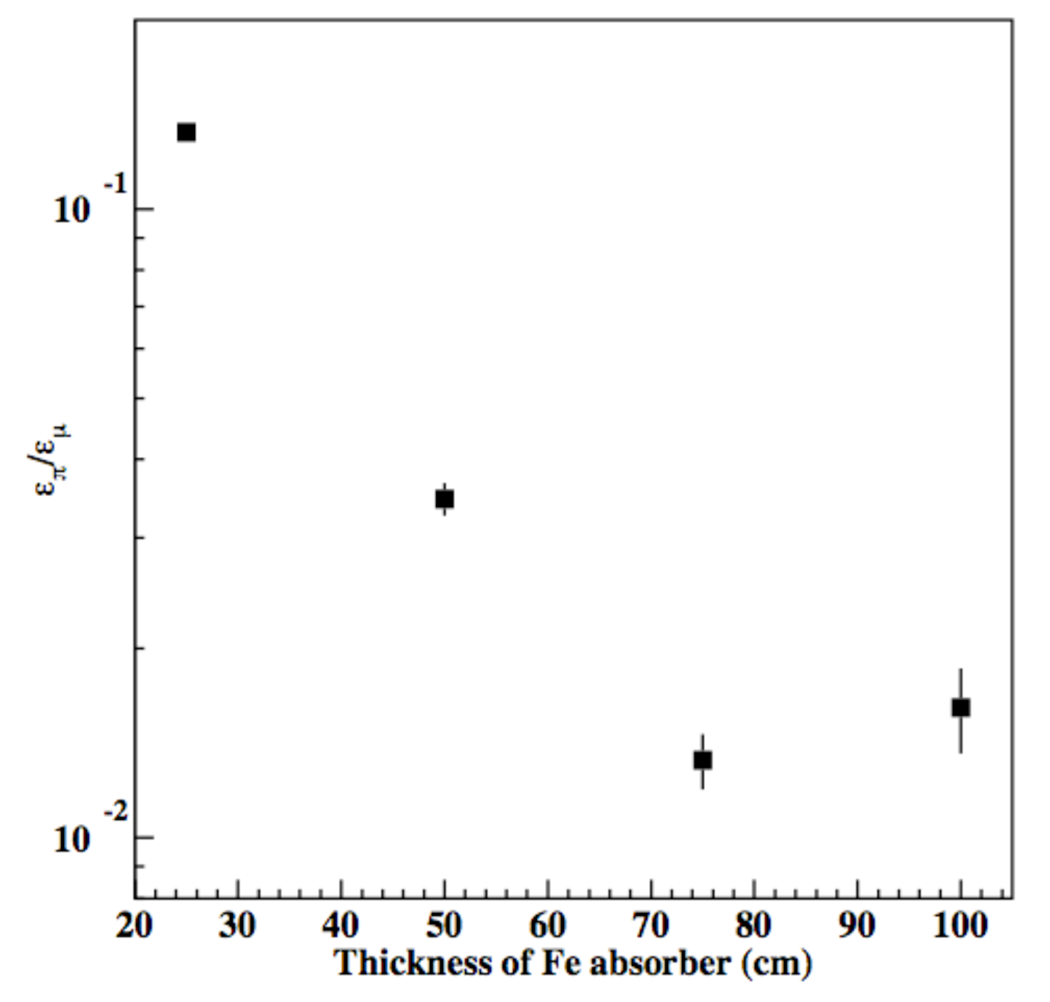
\includegraphics[scale=0.44]{muon/pmrej.pdf}
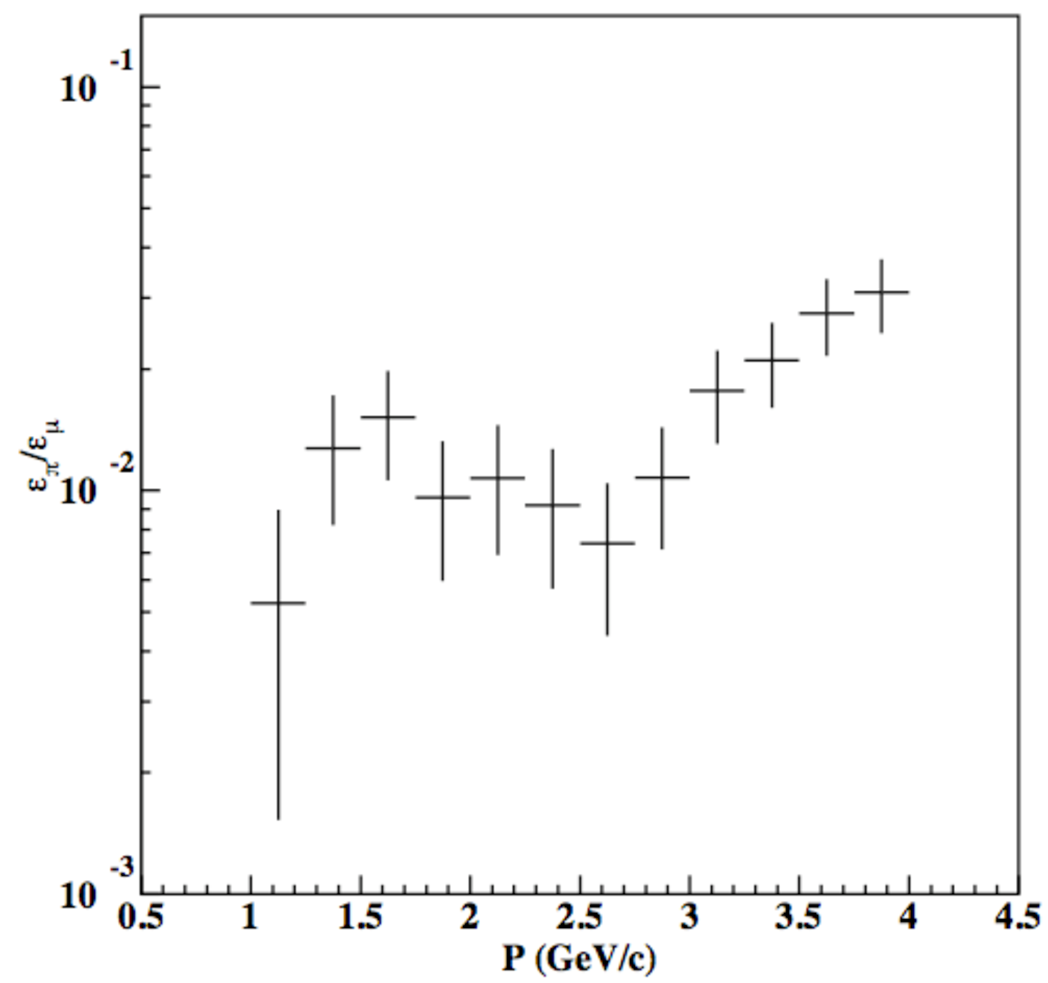
\includegraphics[scale=0.44]{muon/pmrej4.pdf}
\caption{\small{Pion-muon rejection factor $\epsilon_\pi/\epsilon_\mu$ versus total iron absorber thickness
(left) and versus particle momentum for a 75 cm absorber (right).}}\label{fig:pmrej}
\end{figure*}


\subsubsection{Conceptual Design}

On the basis of these simulations, we have designed a muon detector composed of four iron absorbers (total length of $30+15+15+15=75$ cm) 
with a double-layer scintillator hodoscope positioned after each absorber. The muon detector will be mounted behind the ECal.  The front face 
of the first absorber will be at $\sim 180$ cm from the target. Similar to the Ecal, the muon detector will consist of two halves, one above 
and one below the beam plane.  This segmentation is necessary in order to
minimize the effects of the ``sheet-of-flame,'' the multitude of low-energy particles in the horizontal plane, swept into the detector 
acceptance by the dipole analyzing magnet.

The dimensions of the hodoscopes and absorbers are defined using simulations of $A'\to \mu^+\mu^-$. In 
Figure \ref{fig:xymu} the points where muon pairs from $A'$ decays of different masses intercept the ($XY$) plane located at $210$ cm from the 
target are shown. Both muons are required to be detected in the ECal. Overall dimensions of the hodoscopes and absorbers are shown in 
Table \ref{tb:muon}.  
Figure \ref{fig:HPS_view2} shows a CAD
drawing of the HPS detector with the muon system on the right, which includes the 4 absorbers (gray), the vacuum box (light gray) 
between the upper and lower sections, and the final set of scintillator paddles (red). The ECal is directly upstream from the muon detector, 
with its crystals shown in yellow.  In front of the ECal is a large gray vacuum flange.  The silicon tracker is represented by red and gray 
rectangles and  the red point on the left is the target position. The vertical gap between the first hodoscope layers of the two halves is 
about $5$ cm and increases to about $7$ cm for the last layer of hodoscopes. 

\begin{figure*}[!ht]
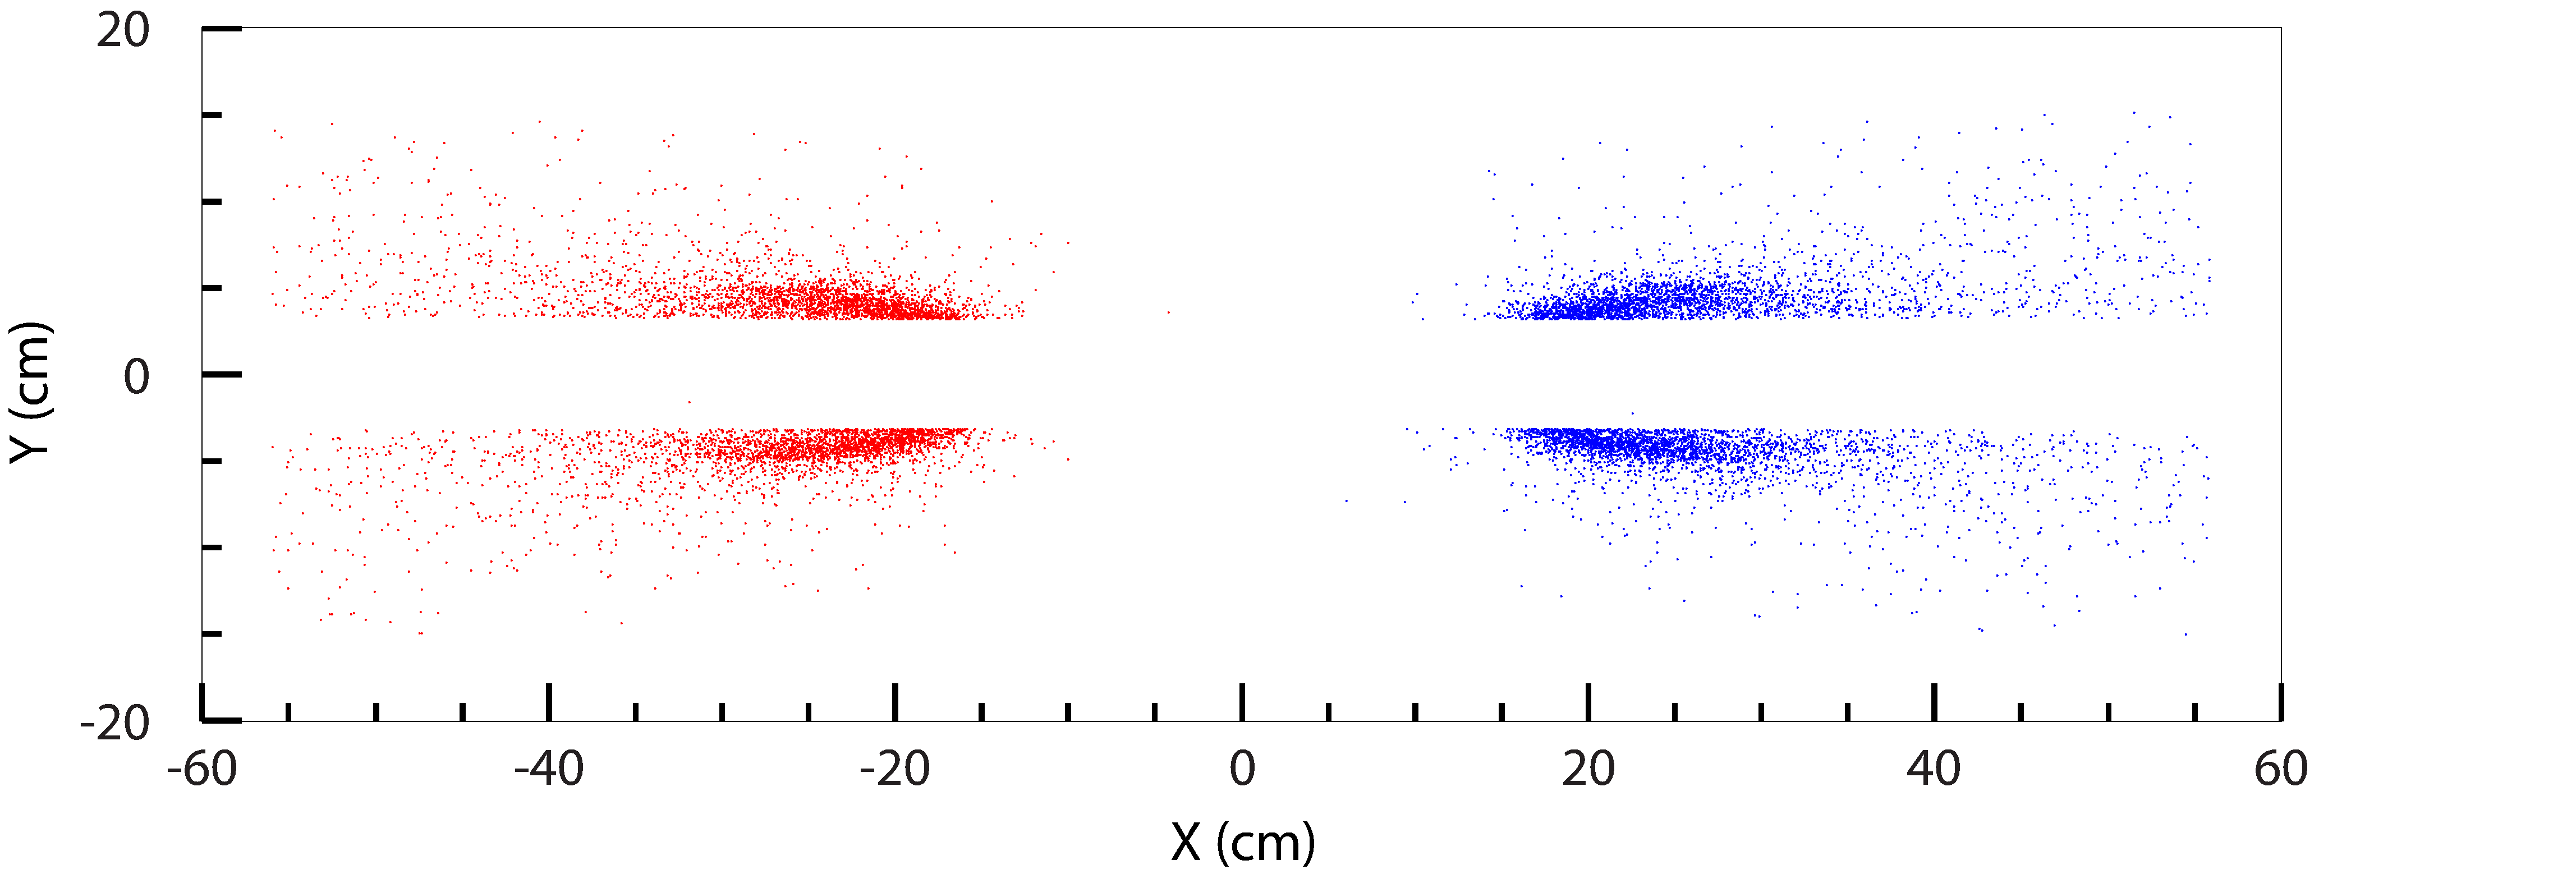
\includegraphics[scale=0.6]{muon/xy_m250.png}
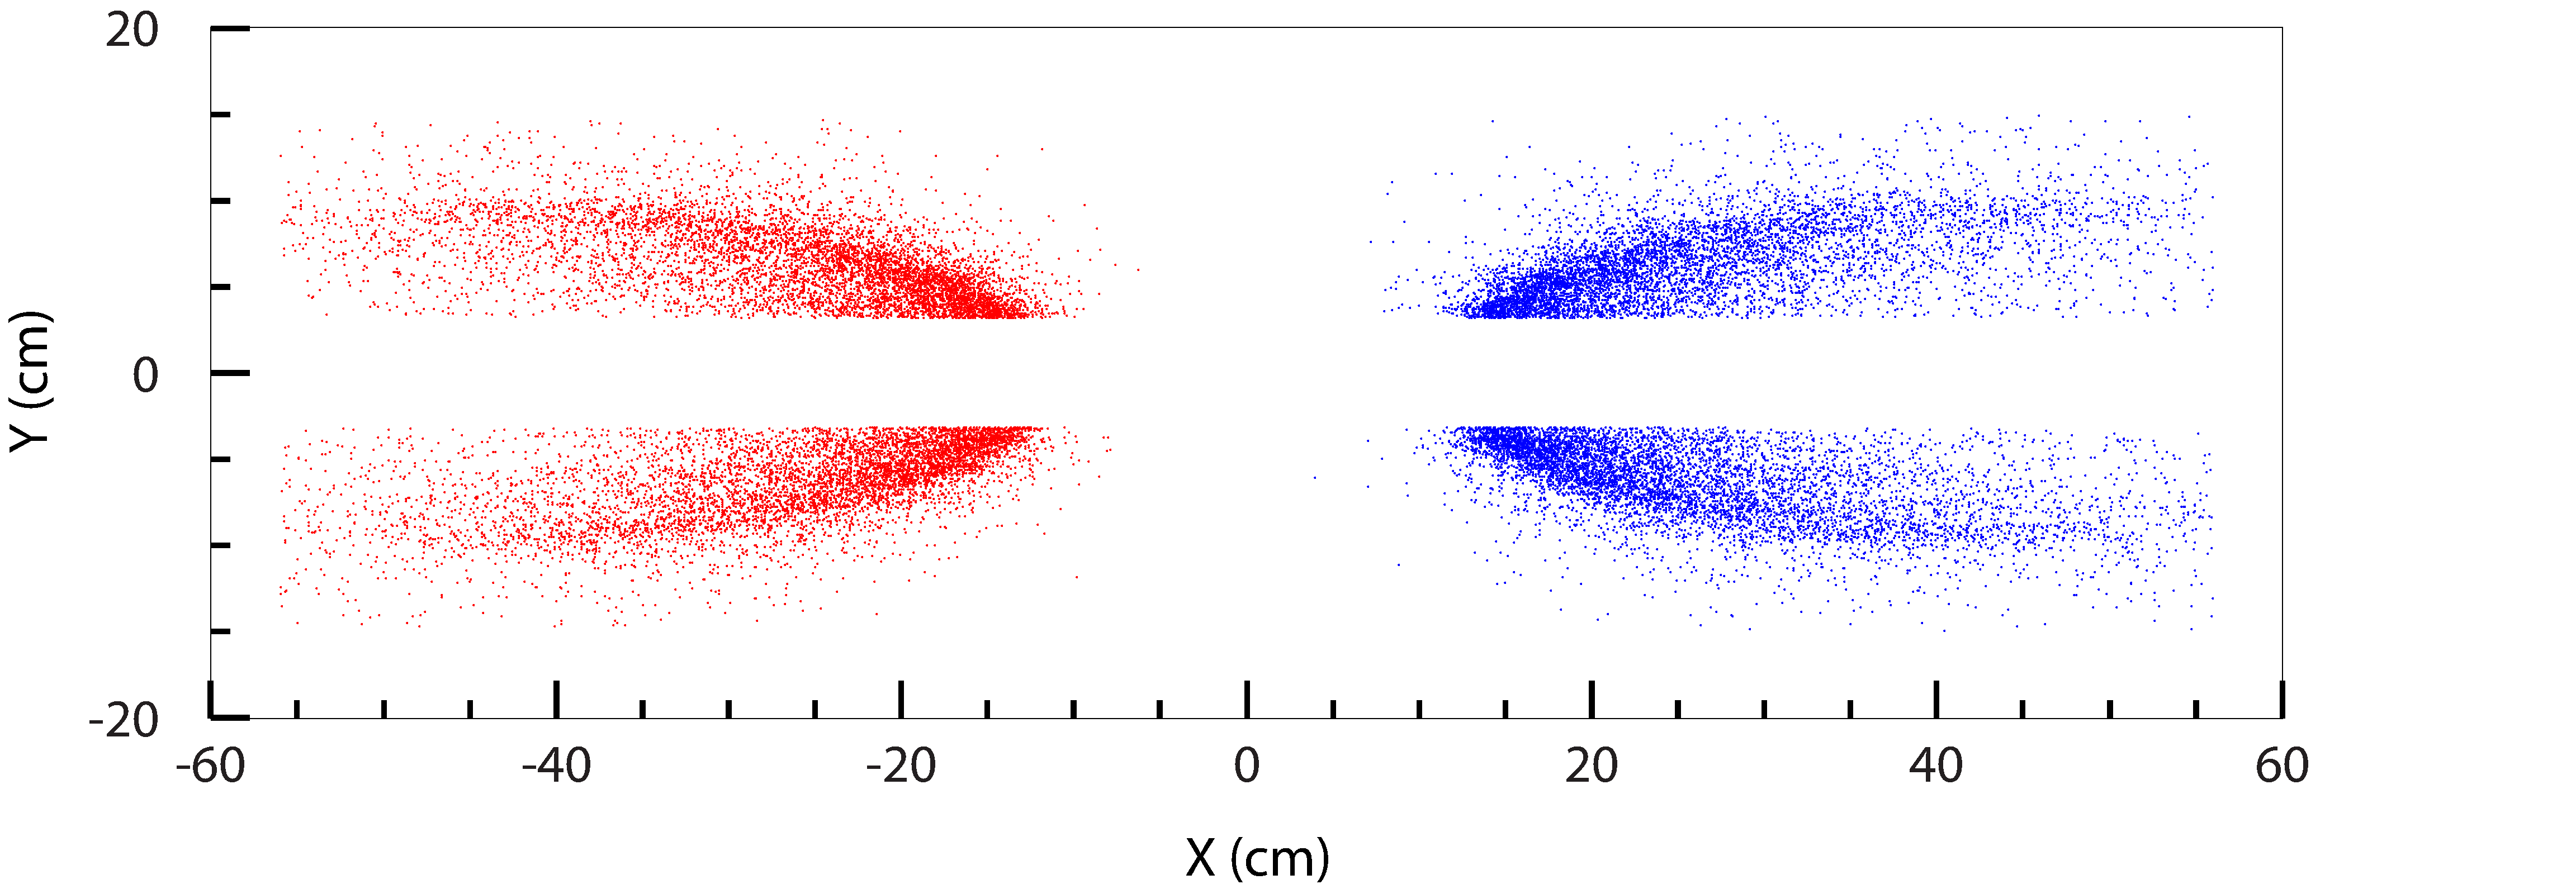
\includegraphics[scale=0.6]{muon/xy_m300.png}
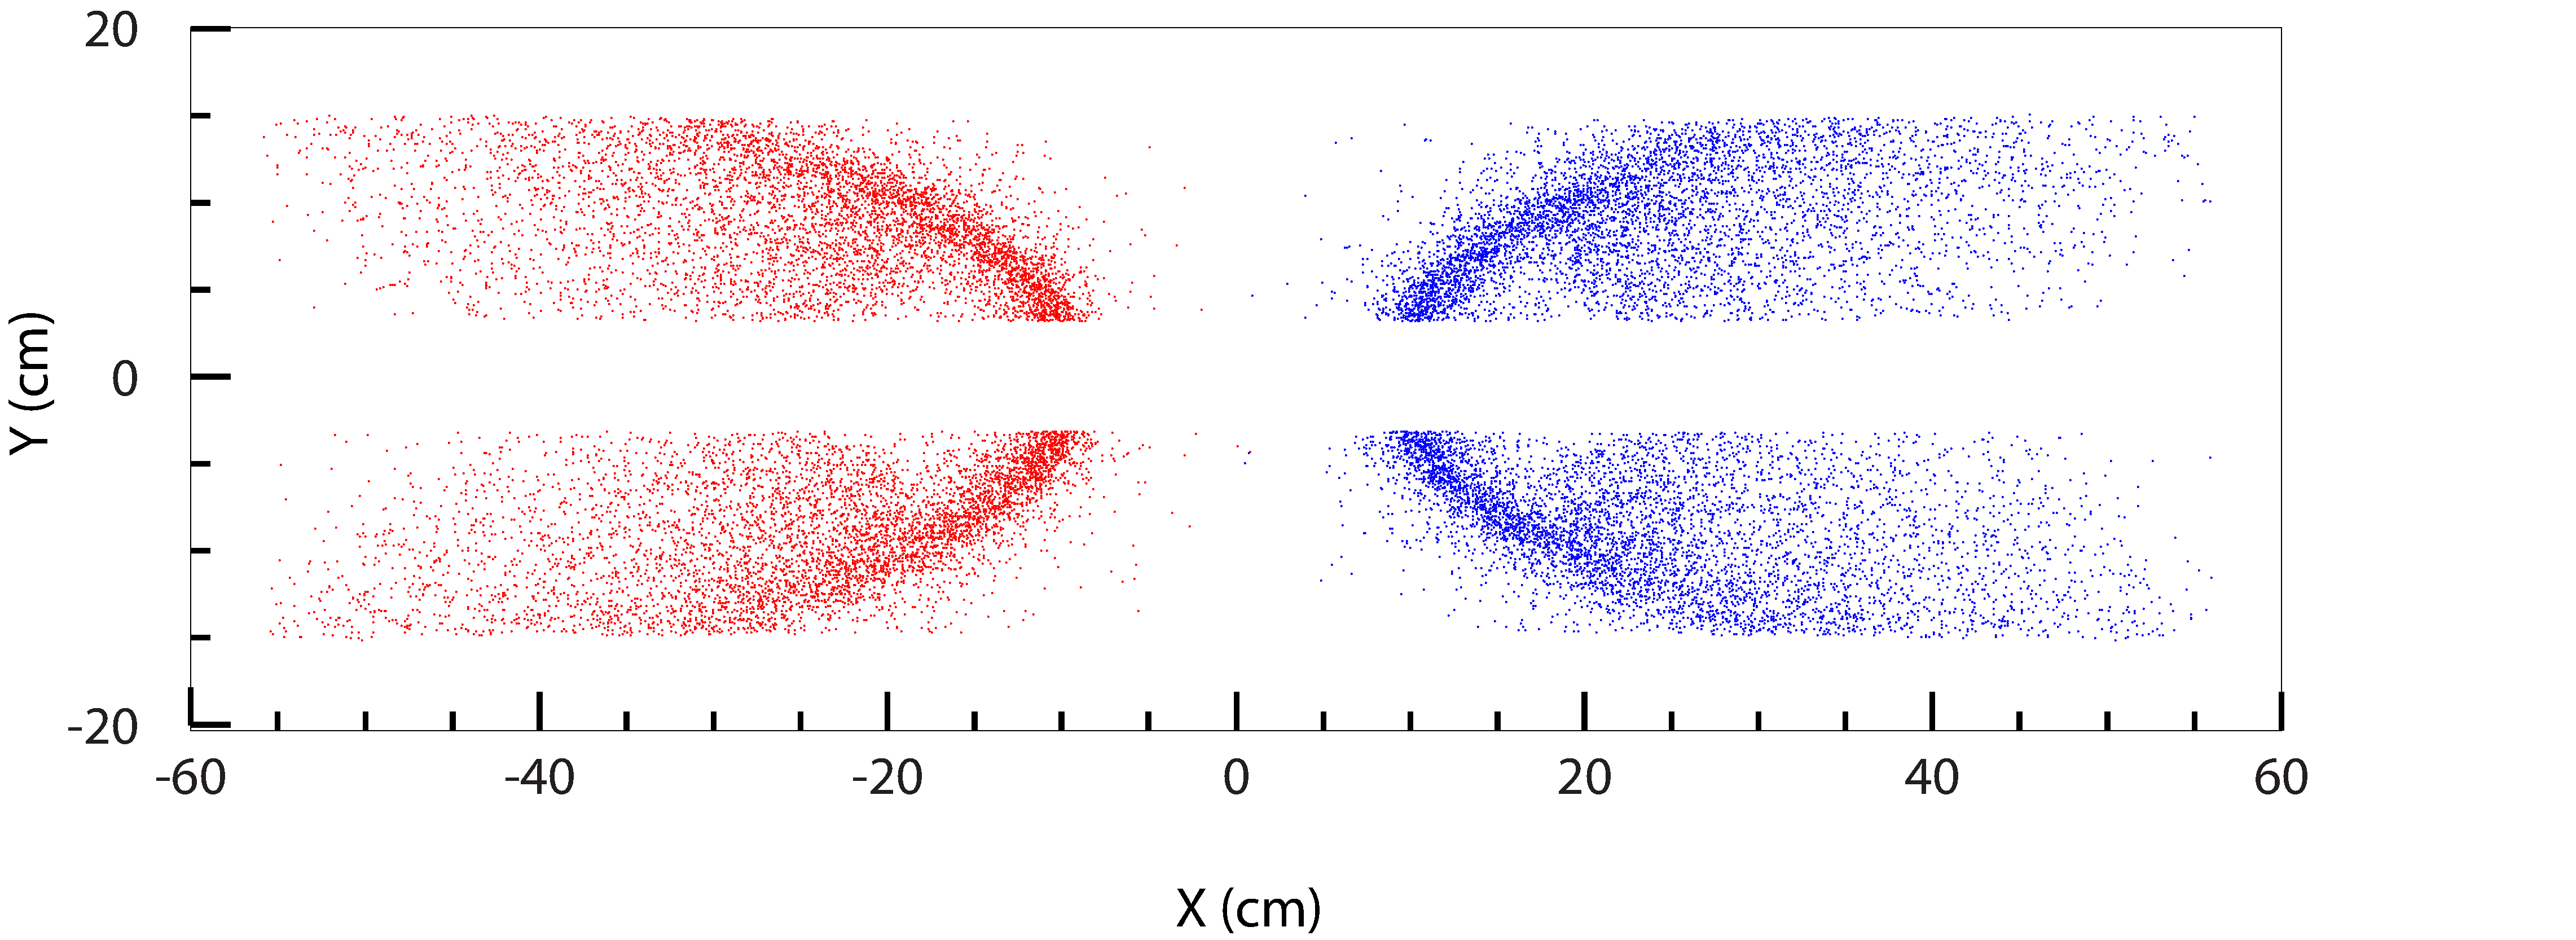
\includegraphics[scale=0.6]{muon/xy_m400.png}
\caption{\small{Points where $\mu^+$ (red) and $\mu^-$ (blue) pairs from $A'$ decays intercept the ($XY$) plane located $210$ cm from the 
target for $A'$ masses $250$ MeV (top), $300$ MeV (middle), and $400$ MeV (bottom.}}\label{fig:xymu}
\end{figure*}

\begin{table}[htdp]
\caption{Dimensions (in cm) of the muon system scintillation hodoscopes (H) and iron absorbers (A). }
\begin{center}
\begin{tabular}{|c|c|c|c|c|}
\hline
&H1&H2&H3&H4\\
\hline
Distance from target& 212&232&252&272\\
Width&112&125&138.5&152\\
Height&10.5&11.5&12.5&13.5\\
\hline
\end{tabular}

\begin{tabular}{|c|c|c|c|c|}
\hline
&A1&A2&A3&A4\\
\hline
Distance from target& 207&227&247&267\\
Width&108.5&122&135&148.5\\
Height&10&11&12&13\\
Thickness & 30 & 15& 15 & 15\\
\hline
\end{tabular}
\end{center}
\label{tb:muon}
\end{table}%


\begin{figure*}[!ht]
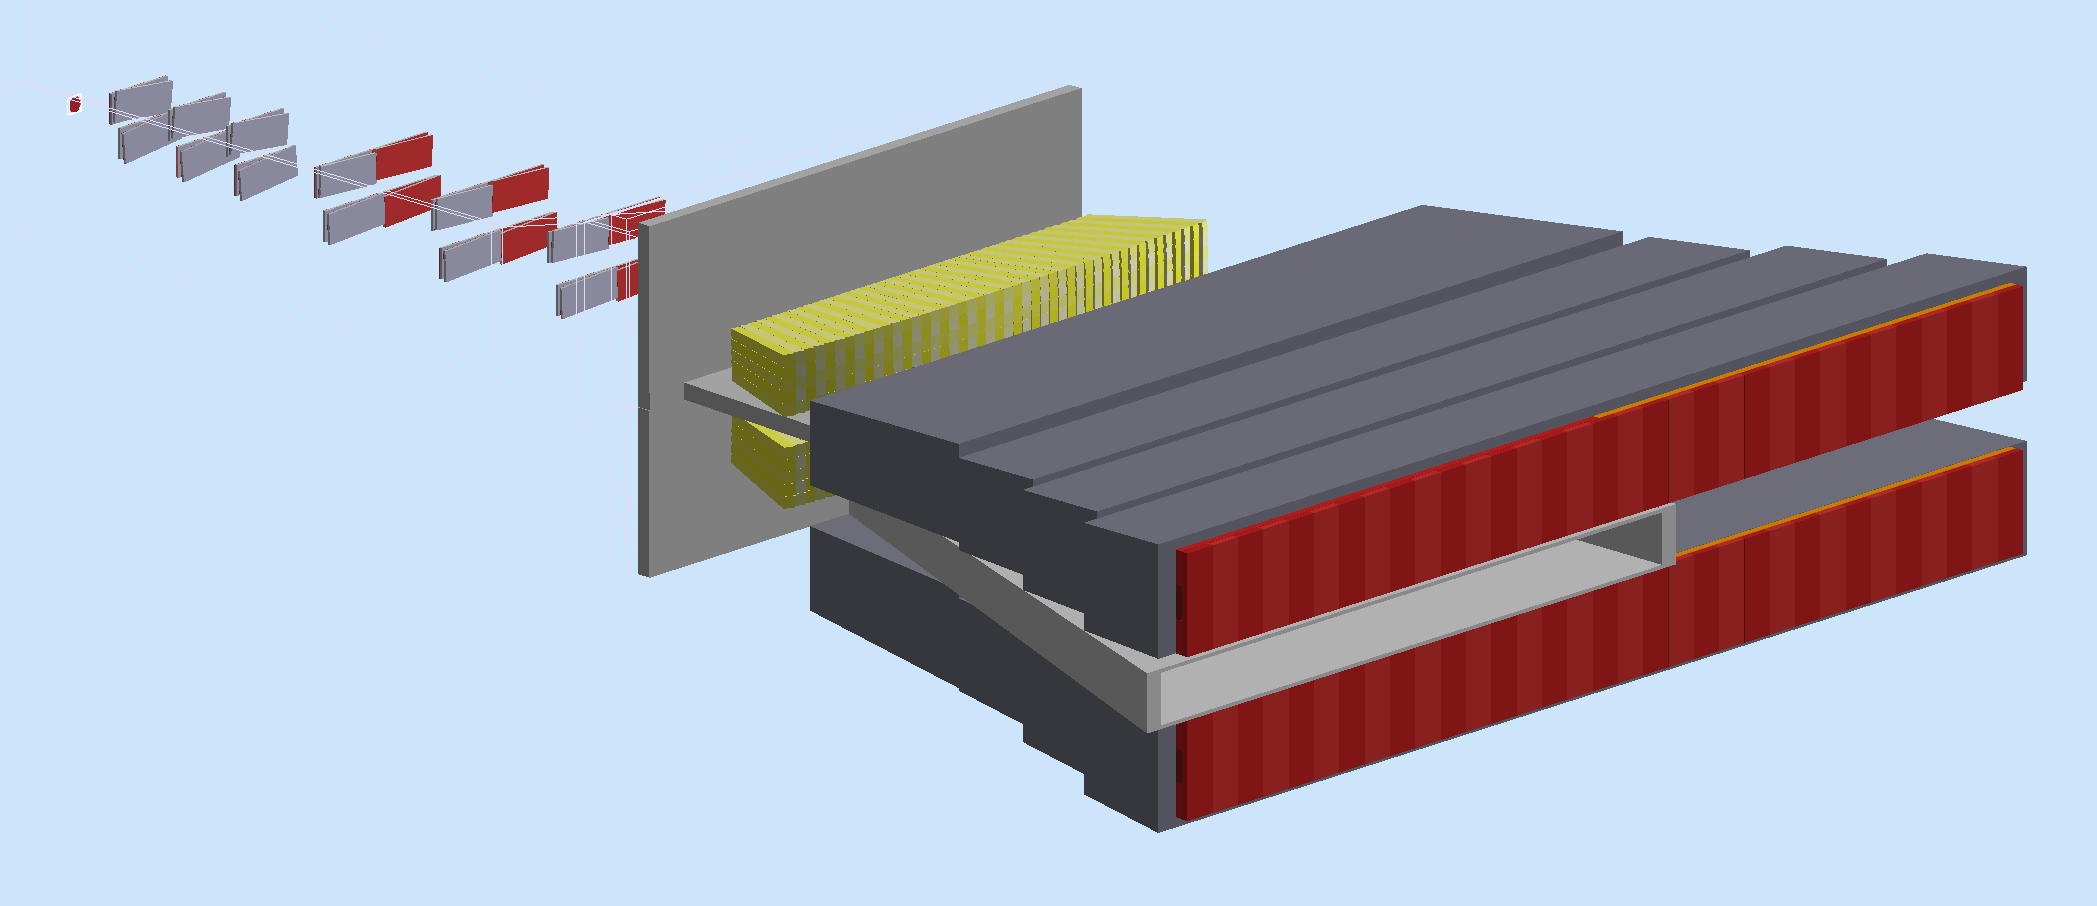
\includegraphics[scale=0.22]{muon/HPS_view2.png}
\caption{\small{CAD drawing of the HPS detector setup.  From left to right this consists of the target (red dot), the silicon tracker
(gray and red rectangles), the large shielding wall (gray), the ECal lead tungstate crystals (yellow, two shades), the muon counter absorbers
(gray), and the final muon counter scintillators (red, two shades).}}
\label{fig:HPS_view2}
\end{figure*}

%\begin{figure*}[!ht]
%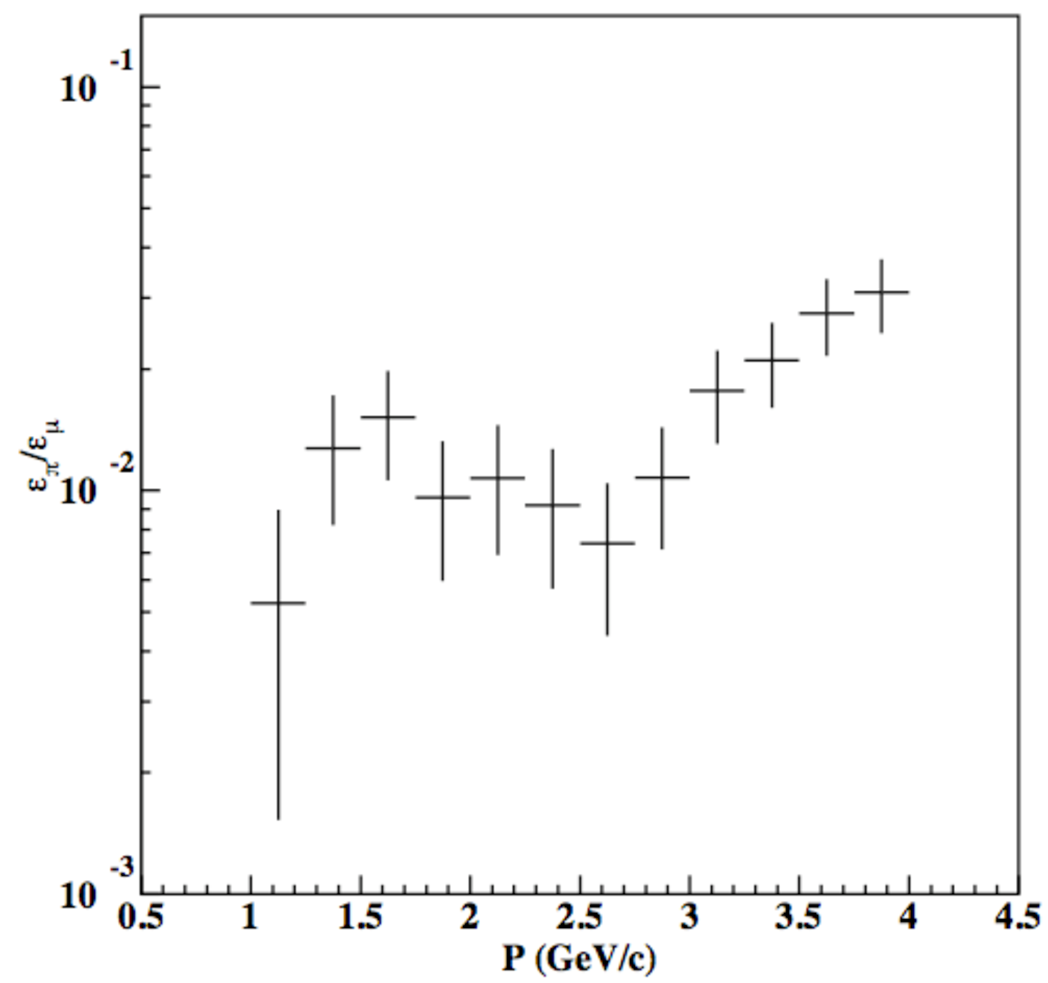
\includegraphics[scale=0.8]{muon/pmrej4.pdf}
%\caption{\small{The pion-muon rejection factor as a function of the iron absorber thickness.}}\label{fig:pmrejp}
%\end{figure*}

\begin{figure*}[!ht]
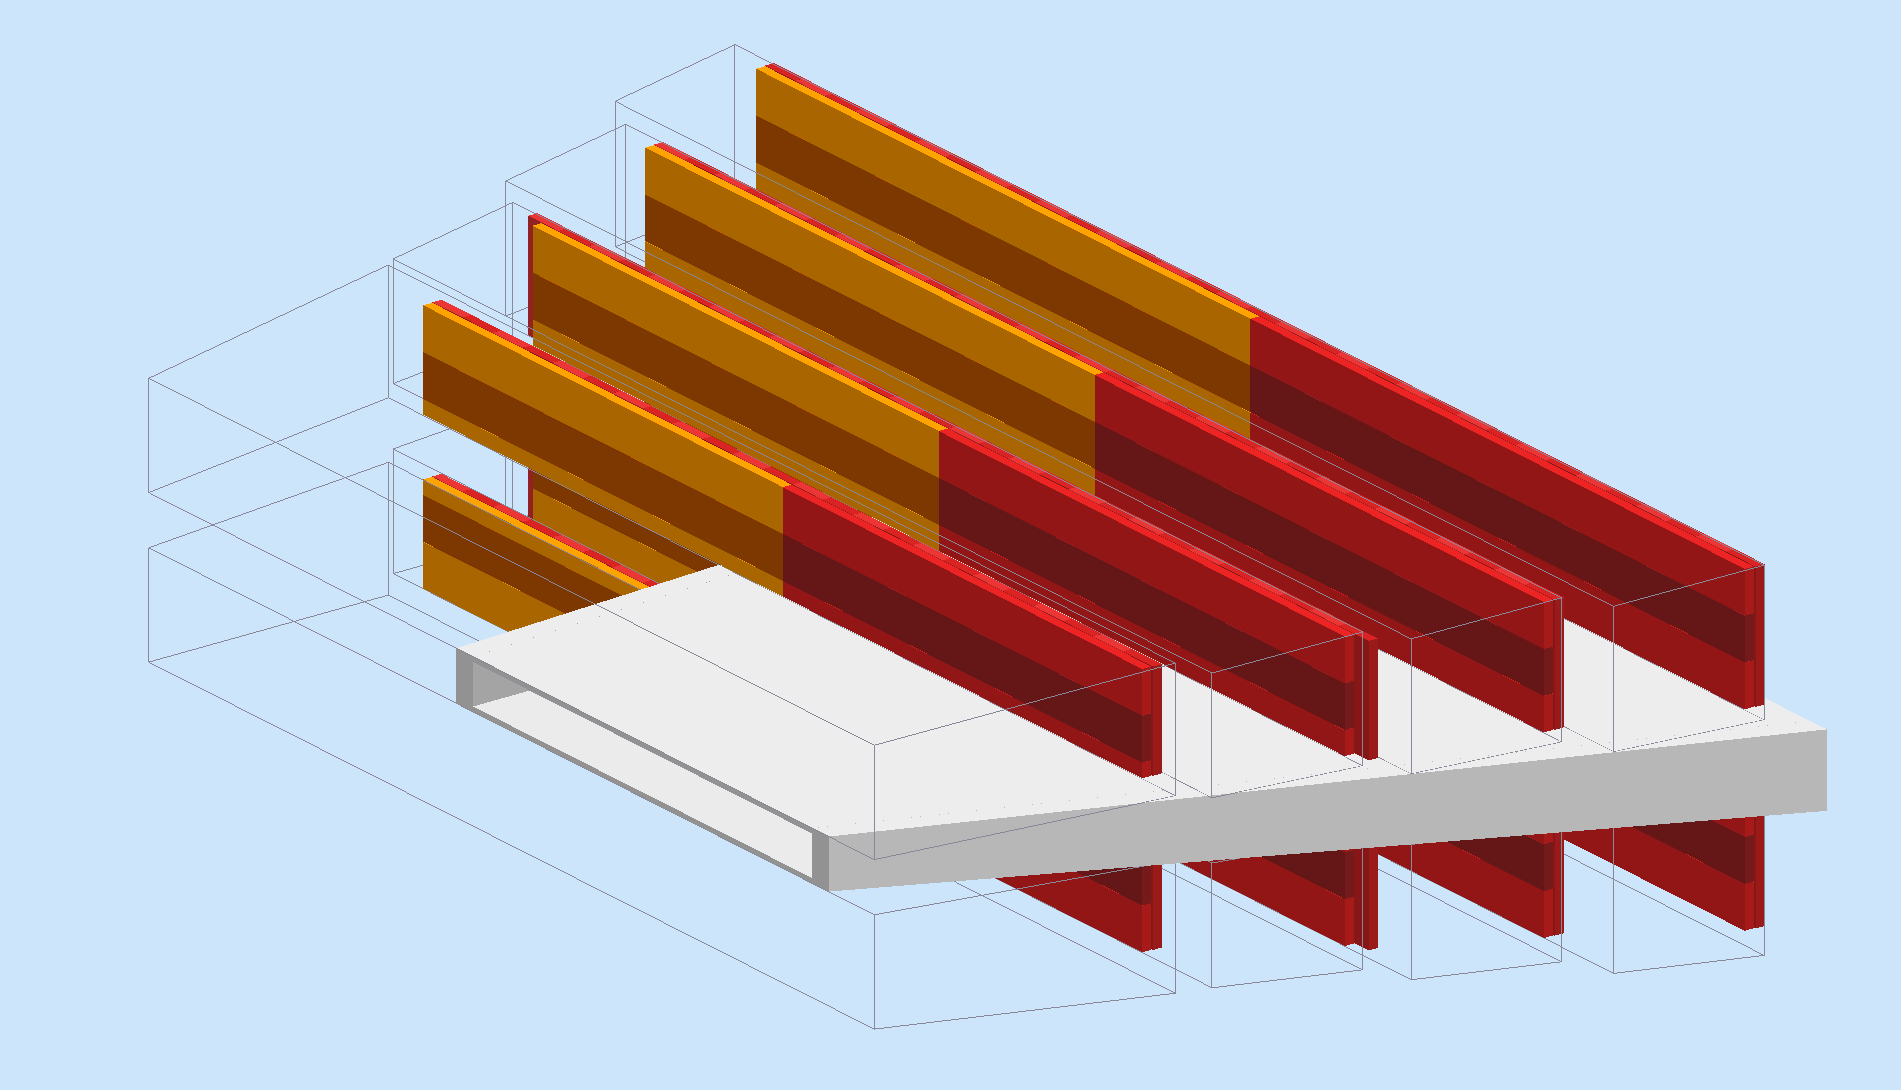
\includegraphics[scale=0.22]{muon/Muon2b.png}
\caption{\small{The horizontal scintillator configuration for the muon counter. Scintillators are
shown in red and yellow/brown.  The white/gray structure is the vacuum box.  Each hodoscope layer (top
and bottom) contains three long strips, read out on both ends.
}}
\label{fig:Muon2p}
\end{figure*}

For the hodoscopes we plan to use the same extruded scintillator strips with embedded wavelength-shifting fiber and phototube readout that was 
developed for the CLAS12 Preshower Calorimeter. These scintillator strips are 45 mm x 10 mm in cross section, and can be cut to any length. 
Widths can be reduced as needed for the muon counter. Each strip contains two long tunnels, created in the original extrusion process, into 
which wave-length shifting fibers can be inserted.  Each hodoscope will consist of one $X$ and one $Y$ plane.  The vertical strips of the last 
hodoscope are shown in two colors in Figure \ref{fig:HPS_view2}. The horizontal counters of the last 
hodoscope plane is shown in
Figure \ref{fig:Muon2p}. The horizontally aligned strips will extend over half the width of the detector and will be read out from the outer ends.  
The upper and lower hodoscopes in each plane will have their own vertically aligned strips, which will be read out only on their outer ends.  
The inner end is inaccessible because of the vacuum box, and there is no particular advantage to having a double readout on these short 
(135 mm) strips.  

The system will be instrumented with less than 256 readout channels so that the requisite electronics will 
fit into a single VME/VXS crate.  The signals from each channel (PMT) 
will be sent to a FADC.  We intend to borrow the CLAS12 Preshower Calorimeter electronics and HV system.  Just as with the ECal, the FADCs will be 
used to construct a muon trigger for the experiment.  In the current design there will be 3 pairs (left-right) of horizontal strips in 
each of 8 hodoscope planes (48 total) and a total of 208 vertical strips in 8 hodoscope planes.  The number of vertical strips per plane 
increases slightly with distance from the target to keep a constant angular coverage.  The maximum is 33 per hodoscope in the back plane.

Full Monte Carlo simulations with realistic event rates are currently under study in order to finalize the design details of the muon counter.  
The crucial issues are the event rates in the scintillators near the beamline (which already has initiated a redesign of the vacuum chamber 
to reduce background), the target-to-muon-counter tracking resolution and the detection efficiency, and the achievable trigger rates.  
Any changes to the detector as a result of these studies are expected to be minor and will not alter the conceptual design presented here.

\subsubsection{ $\mu^+\mu^-$ Trigger} 

%The muon trigger will look for an energy deposition consistent with that of a MIP particle in single ECal channels and in the muon hodoscopes from a $\mu^+\mu^-$ pairs.  The CTPs in the three VXS crates (two for each half of the ECal and one for the Muon System) will search for MIP hits using energy selections on the hits reported by the FADCs satisfying: $E_{MIP}^{min}<E_{ECal\_channel}<E_{MIP}^{max}$ for the ECal and $E_{MIP_thr}<E_{\mu\_hodo}$ for the Muon System. The CTP in the Muon System will use time information of the reported MIP hits to select coincidences in three planes of each hodoscope layer according to the geometry of horizontal and vertical strips. After the MIP hits in the ECal and in the muon system are selected, the CTP sends the time and position information of each selected hit to the SSP. The SSP will look for time and position coincidence of MIP hits in the ECal with hits in at least the tthree first layers of the Muon System, treating the top and bottom halves of the detector separately. To form the final $\mu^+\mu^-$ trigger decision it will select pairs of MIP hits in opposite quadrants of the detector (similar to the coplanarity requirements described above) that are within a programmable coincidence time window. 

The muon trigger will look for 
$\mu^+\mu^-$ pairs by finding energy depositions consistent with those expected from minimum ionizing particles in the layers of the muon system.  
The trigger algorithm in the CTP of the muon system  VXS crate will produce a muon pair trigger in four steps:
\begin{itemize}
\item search for MIP hits using energy selections on the hits reported by the FADCs which satisfy $E_{MIP}^{thr}<E_{\mu\_hodo}$
\item use the time information of the reported MIP hits to select coincidences between the two planes of each hodoscope layer, quadrant by quadrant.  
\item look for coincidences in successive quadrants of at least the first three layers of the muon hodoscopes 
\item select pairs of triple coincidences in opposite quadrants of the detector and report the times and positions of coincident triple hits 
to the SSP 
\end{itemize}
If it is necessary to reduce the rate further, the SSP can in addition look for time and position coincidences of MIP hits in the ECal, defined in the ECal 
crate CTPs as hits with 1 or 2 crystals and energy within predefined thresholds: $E_{MIP}^{min}<E_{ECal\_channel}<E_{MIP}^{max}$. 
The SSP will send the final decision regarding the $\mu^+\mu^-$ trigger to the Trigger Supervisor  board. 

\subsubsection{Muon system trigger rates}
\label{sec:muontrigg}

Like the ECal, the muon system trigger rates are dominated by beam backgrounds.  
A GEANT4 model of the HPS detector was used to estimate the rates, following the conceptual design for the muon system presented in 
Section\ref{sec:muon}. Figure \ref{fig:HPS_view2} shows the layout of the system. Each of eight hodoscope layers (four layers in 
the top part of the detector and four in the bottom) consists of two planes of scintillator strips. One plane, called the Y-plane, has strips 
oriented horizontally. The other, called the X-plane, has them oriented vertically. The Y-strips are segmented exactly in the middle
and outside ends, left or right, are read out. 
Six Y-strips make up each half plane, so the total number of Y-strips is 48. 
X-planes are divided into 4.5 cm wide segments, with 240 strips in total. It should be noted that the number of vertical strips 
in the conceptual design is only 208 to limit the total number of readout channels to 256, one crate's worth. Since the rates in the 
vertical strips at the edges of the hodoscope are very low, eight strips in each 
plane can be paired to make four readout channels without negatively impacting the detector occupancy. In Table \ref{tb:muonstrp}, 
the lengths and widths of the detector readout segments (counters) used in the simulation are presented. There is a $14$ cm wide 
and $3.5$ cm high gap 
introduced into the model, centered on the point where the electron beam passes through the muon vacuum chamber, to avoid the high rate region.
As shown in Figure \ref{fig:xymu} 
this gap has a negligible effect on the detection efficiency of muon pairs from $\ap$ decays. 

\begin{table}[htdp]
\caption{Lengths and widths of the hodoscope strips. Dimensions are centimeters.}
\begin{center}
\begin{tabular}{|c|c|c|c|c|}
\hline\hline
Readout plane& Layer 1&Layer 2&Layer 3& Layer 4 \\
\hline
X-plane width& 4.5& 4.5 & 4.5 & 4.5  \\
X-plane length&10.5&11.5&12.5&13.5\\
\hline
Y-plane width& 3.5 all three&3.5, 4, 4  & 3.5, 4.5, 4.5 & 4.5 all three\\
Y-plane length&56&62.5&70&76\\
\hline\hline
\end{tabular}
\end{center}
\label{tb:muonstrp}
\end{table}%

Events generated in EGS5 were used as an input to the GEANT4 simulation. The CEBAF beam bunch structure was simulated by sending 
one bunch equivalent of electrons, 5,625 $e^-$'s (6.6 GeV), through 
the target to generate secondaries and scattered beam particles. The secondaries were followed through the apparatus
to simulate the detector response. As expected, the 
highest background rates are seen in the Layer 1 hodoscope and are $\sim 0.7$ MHz in both the X-strips near the electron beam location and 
the beam-left Y-strip closest to the beam plane, see Figure \ref{fig:l1rates}. Rates in the vertical strips far from the 
beam position are very low, allowing multiple strips to be combined into a single readout channel in order to reduce the number 
of PMTs and electronic channels.  

\begin{figure}[htbp]
\begin{center}
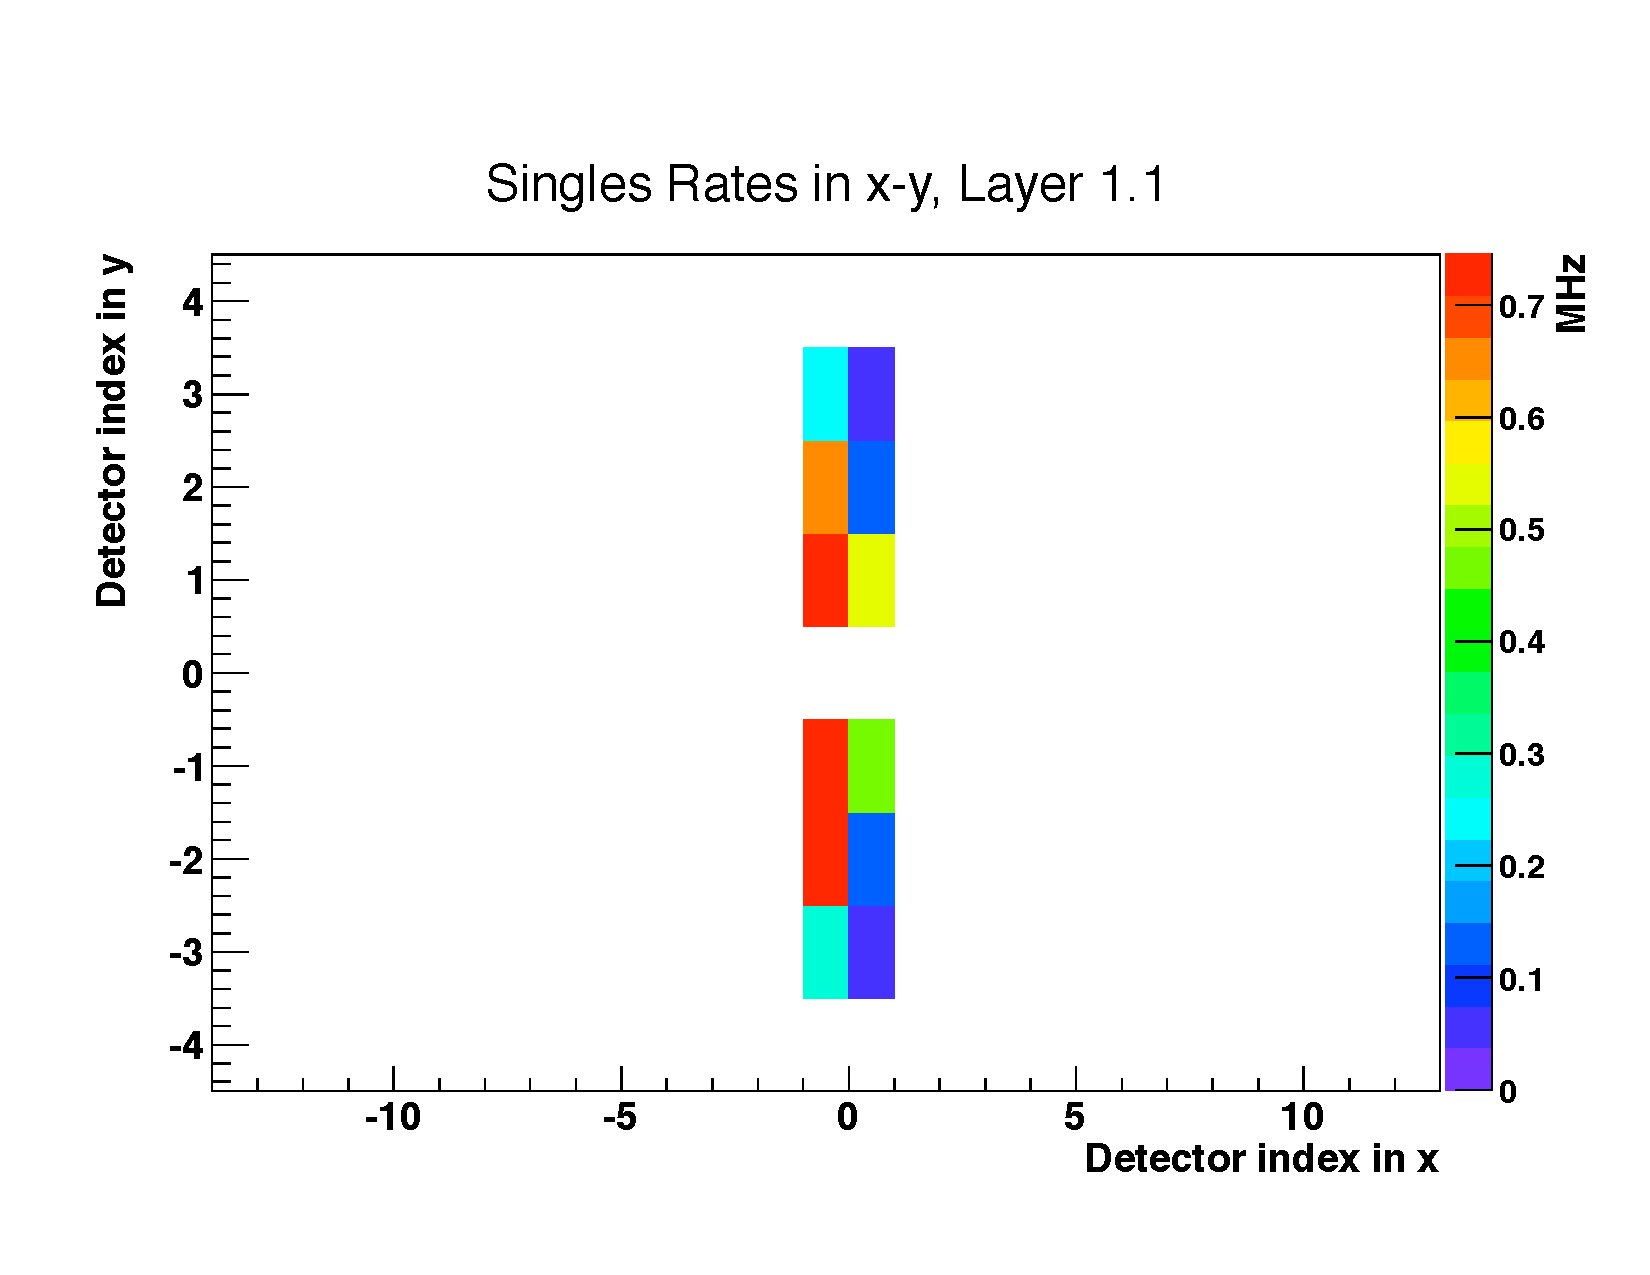
\includegraphics[width=0.475\textwidth]{performance/trigger/muon_singles1}
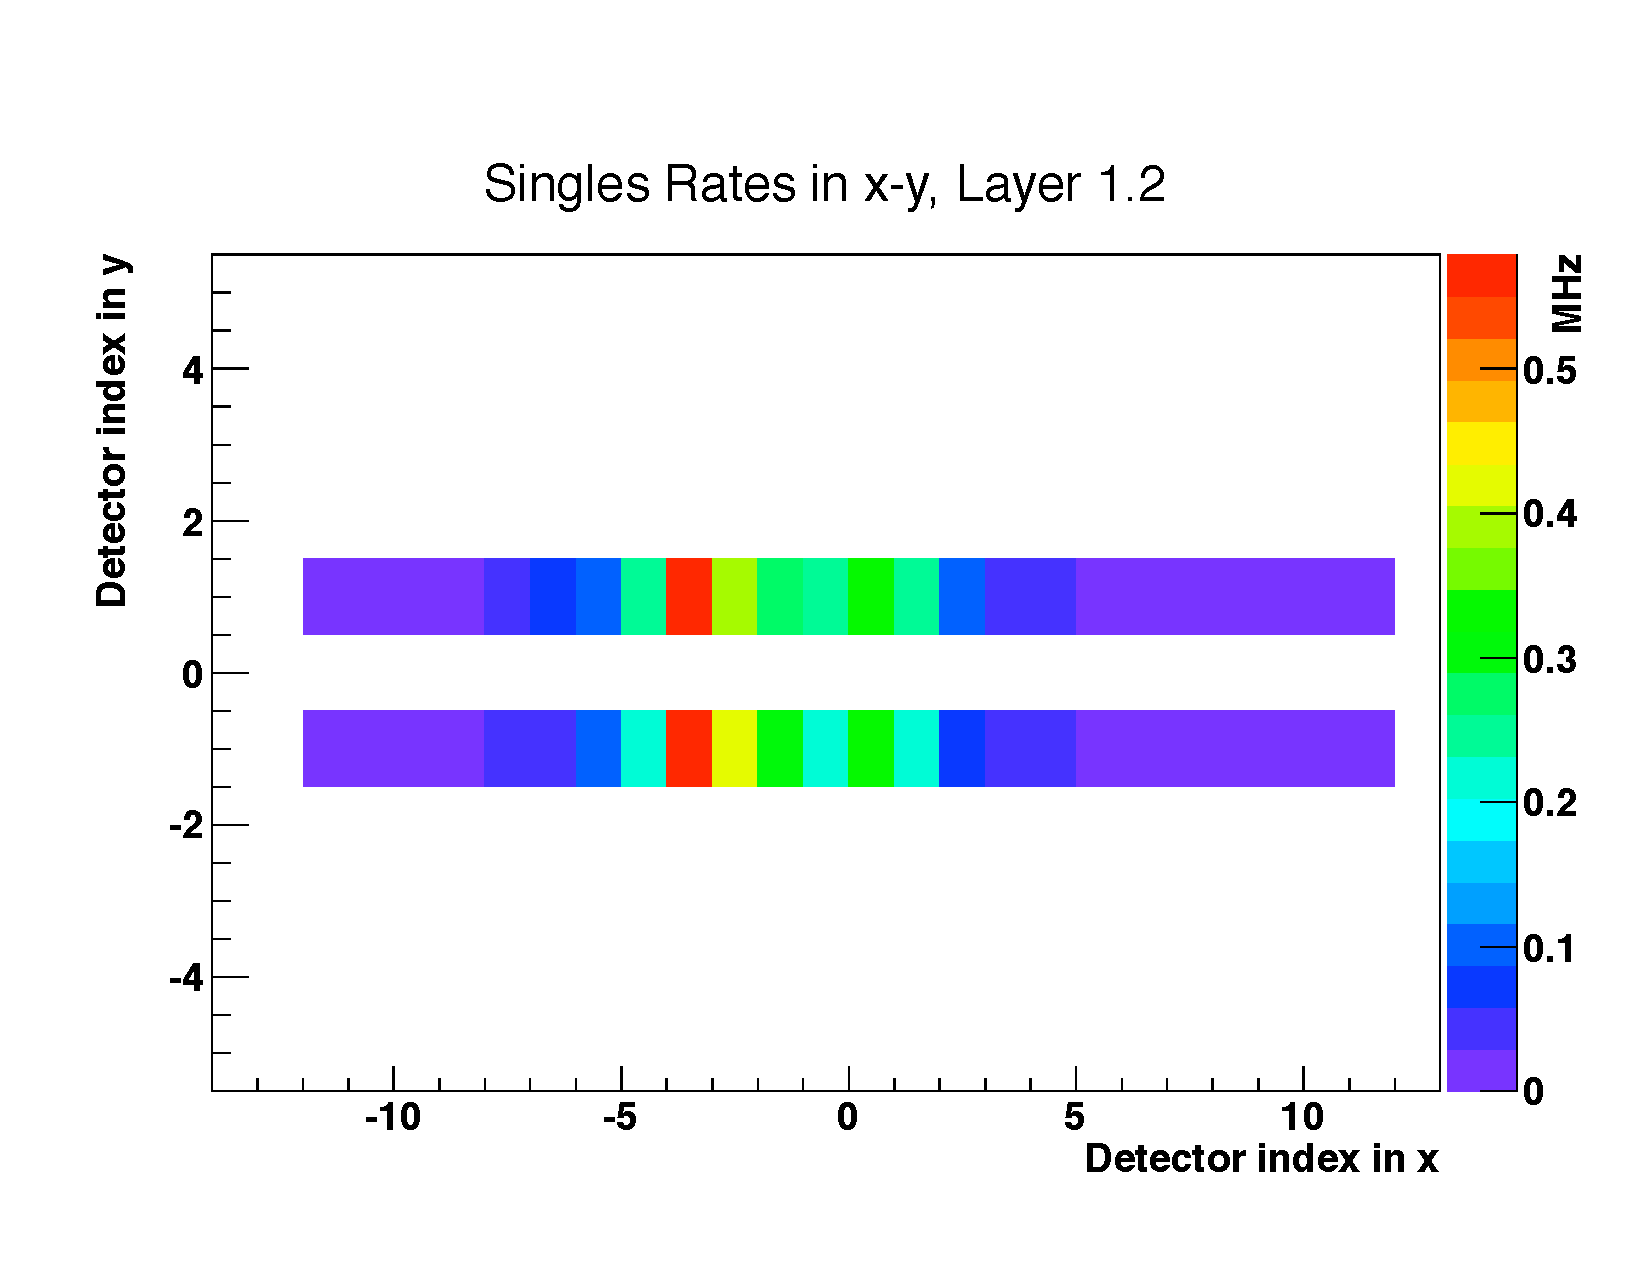
\includegraphics[width=0.475\textwidth]{performance/trigger/muon_singles2}
\caption{Rates in Y- (left) and X-planes (right) of the Layer 1 hodoscopes for hits with energy deposition $> 0.5$ MeV.}
\label{fig:l1rates}
\end{center}
\end{figure}

The coincidence rates between hodoscope planes in a given layer and between different layers have been studied using a $16$ ns coincidence 
time window. 
On the left of  Figure \ref{fig:c1rates}, the coincidence rates between X- and Y-quadrants, top-left (TL), top-right (TR), bottom-left 
(BL), and bottom-right (BR) of the Layer 1 hodoscope are shown. On the right, the figure shows coincidence rates of respective 
quadrants of Layers 1 and 2. The fact that there is a significant reduction of the rates from 2-plane (~1.2 MHz) to 2-layers (0.07MHz) 
coincidences indicates that hits are mostly from uncorrelated background. For the muon trigger, a coincidence of two opposite quadrants 
(TLxBR) or (TRxBL) is required along with triple coincidences of the first three layers of hodoscopes in each quadrant. The rates of the 
triple quadrant  
coincidences within $16$ ns are shown in Figure \ref{fig:c3rates}. The maximum trigger rates are in the beam-right (electron side) 
quadrants and are on order of $7$ kHz. In the beam-left quadrants (positron side), the tripple coincidence rates are $<1$ kHz. 
Since an overall trigger requires hits in two opposite quandrants, the maximum 
rate will be $<1$ kHz. While a further reduction of rates will be possible with the inclusion of 
MIP hits in the ECal, the $<1$ kHz is a small addition to the total trigger rate from the Ecal trigger (see discussions in 
Section \ref{sec:ecaltrigg}) and will keep overall trigger rate well within the limit of allowed rates for the HPS DAQ.   

\begin{figure}[htbp]
\begin{center}
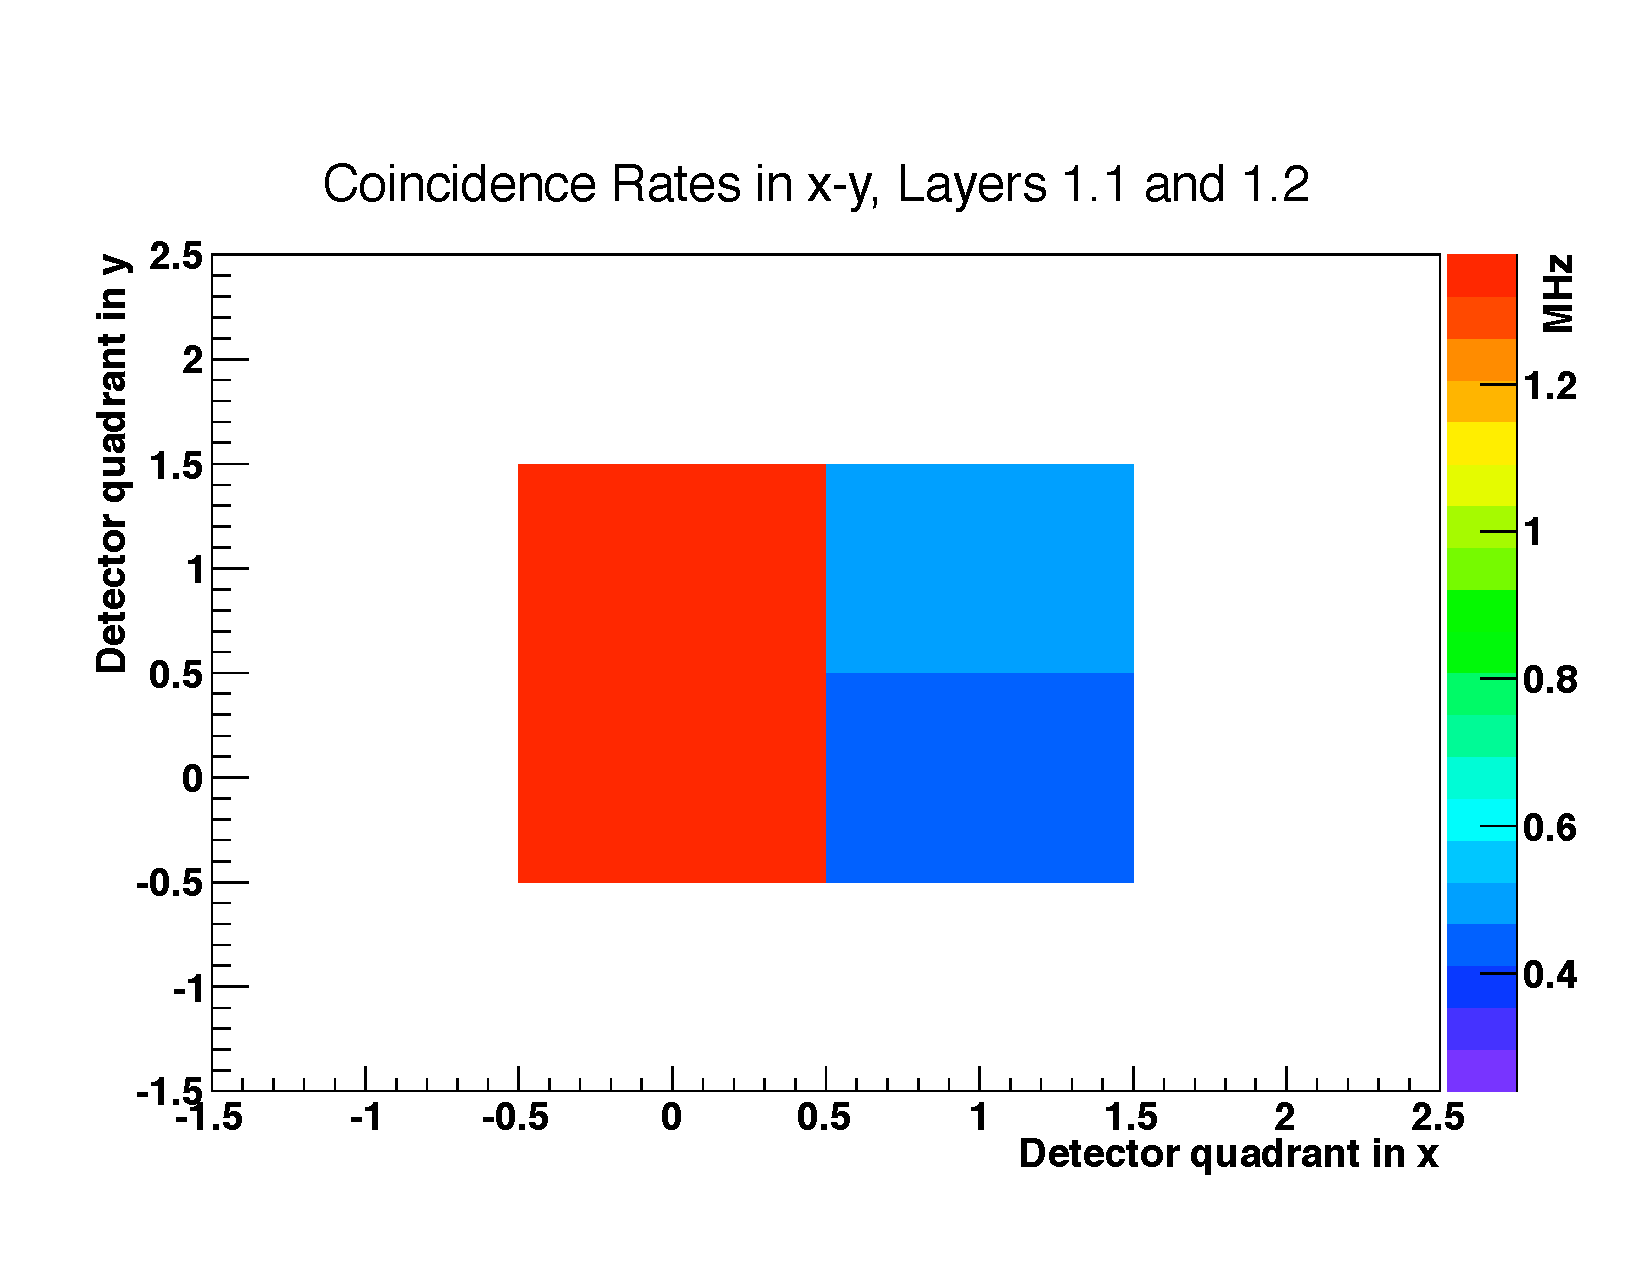
\includegraphics[width=0.475\textwidth]{performance/trigger/muon_coinrate1}
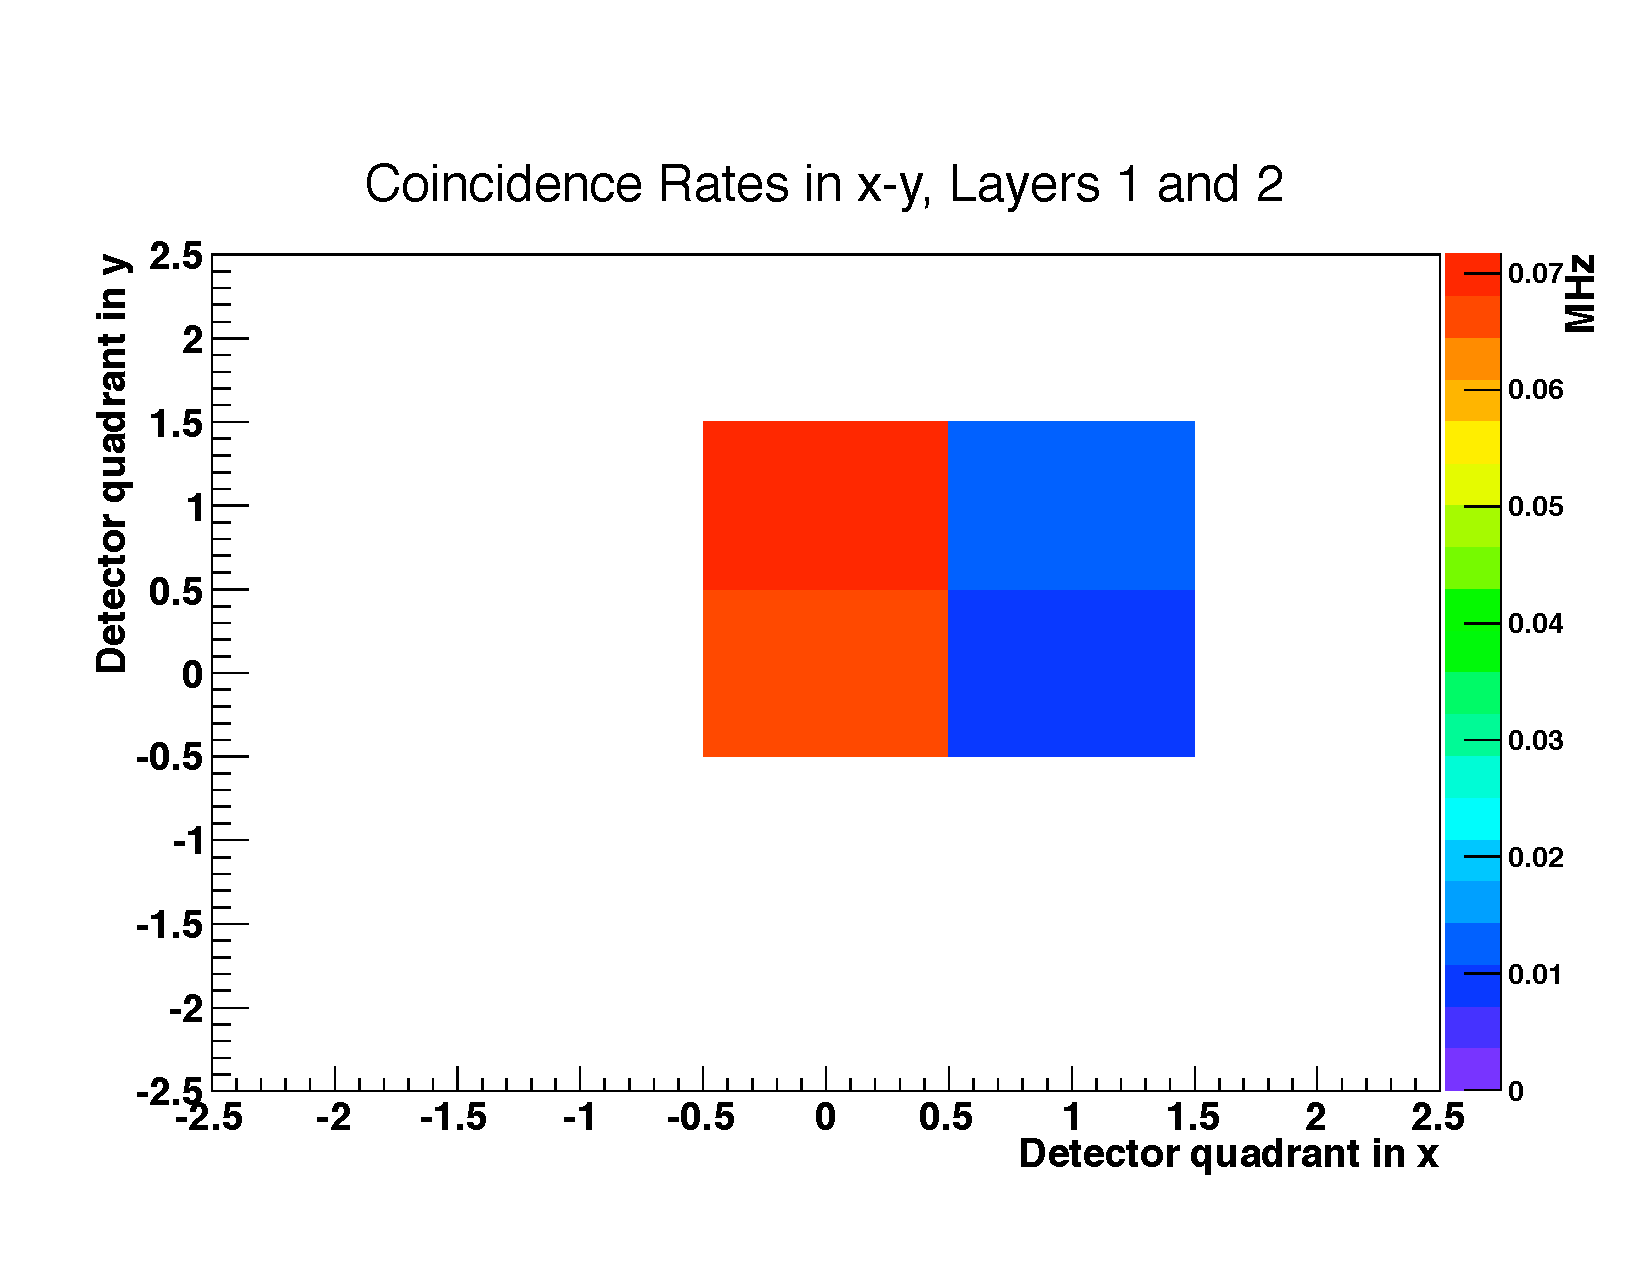
\includegraphics[width=0.475\textwidth]{performance/trigger/muon_coinrate2}
\caption{Coincidence rates between X- and Y-quadrants of the Layer 1 hodoscope (left graph) and coincidence rates between Layer 1 and 2 
(right graph). }
\label{fig:c1rates}
\end{center}
\end{figure}

\begin{figure}[htbp]
\begin{center}
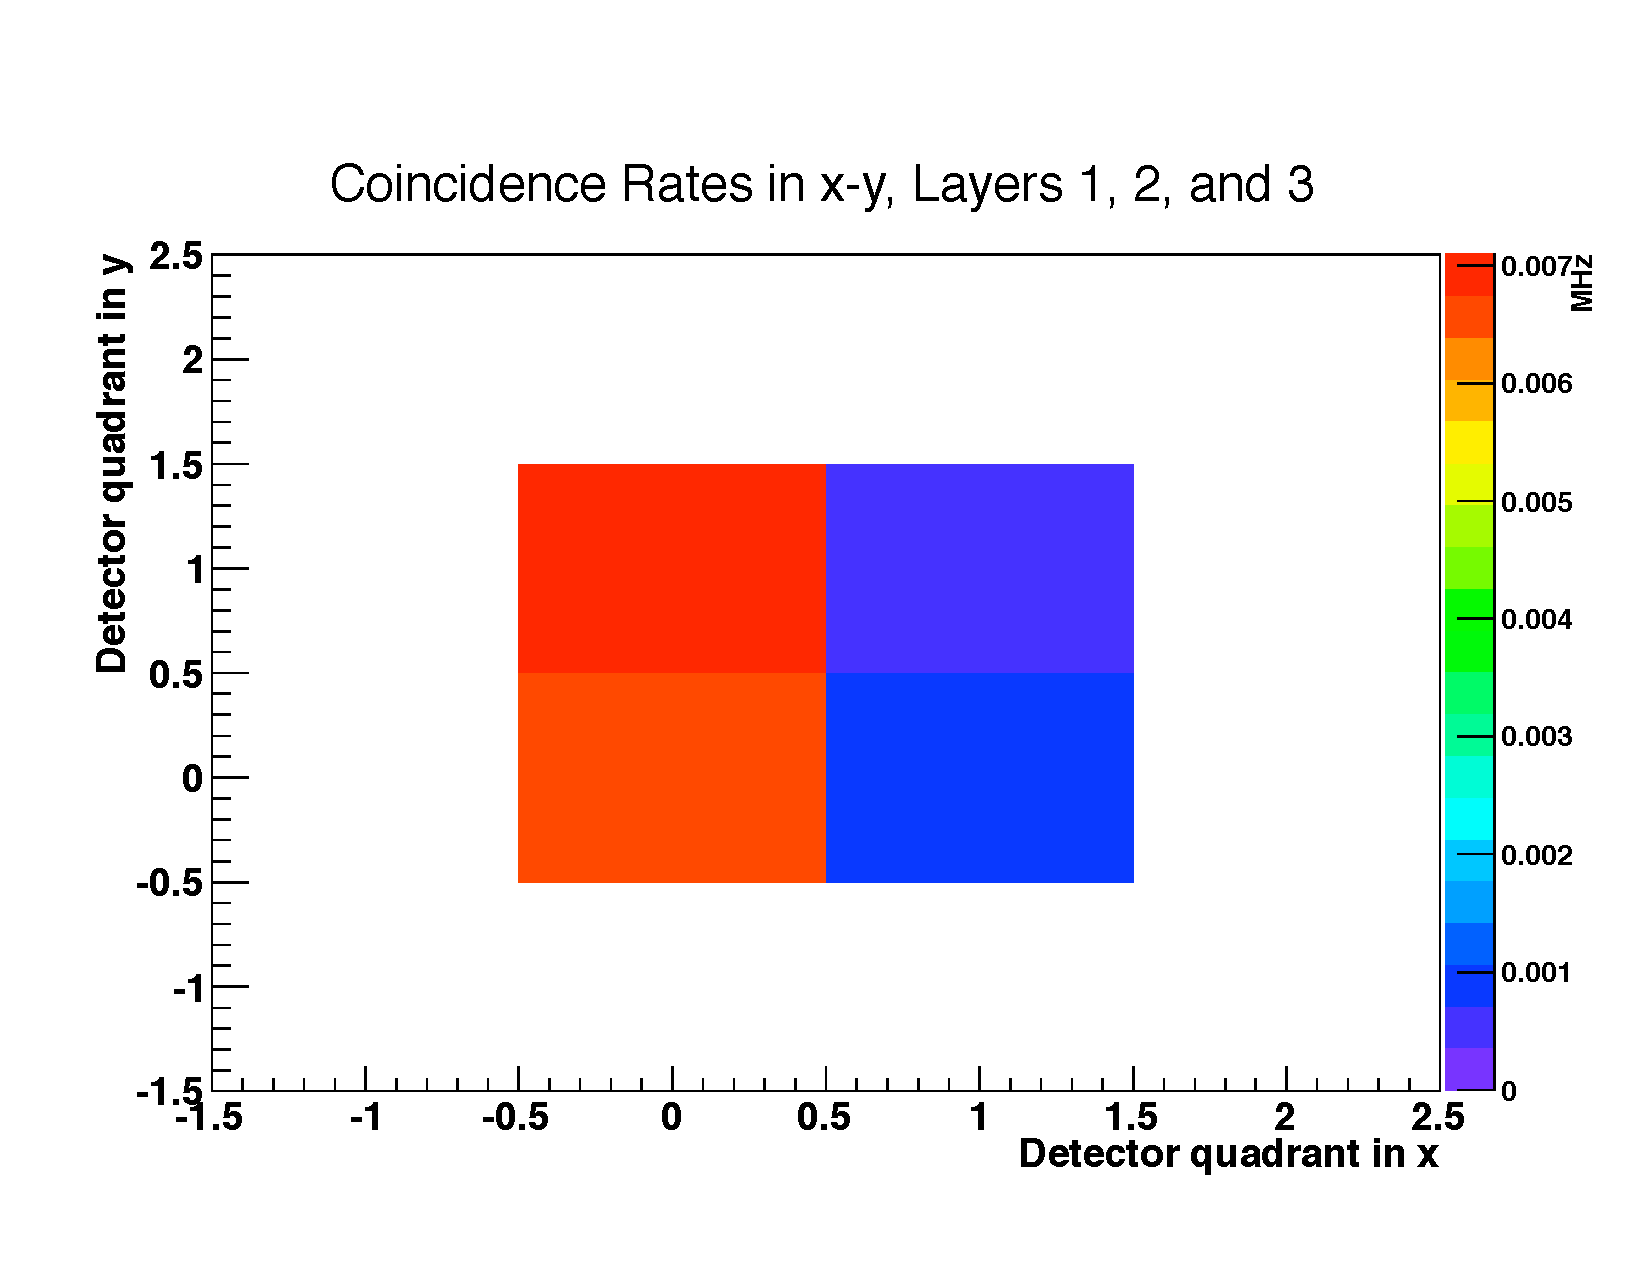
\includegraphics[width=\textwidth]{performance/trigger/muon_coinrate3}
\caption{Coincidence rates in first three layers of muon hodoscopes. The coincidence time window is set to $16$ ns. }
\label{fig:c3rates}
\end{center}
\end{figure}







